%\documentclass[danish, a4paper, twocolumn, oneside]{memoir}
%\usepackage{A1_preamble}
\documentclass[A2_main.tex]{subfiles}

\begin{document}
\section{Databehandling}
\subsection{Grundfrekvensens afhængighed af snorspænding}
Her foretages varibel kontrol. $\mu$ og $L$ i \cref{eq: wave}. Observationerne kan ses i \cref{fig:frekvensSNor}.
\begin{figure}[H]
    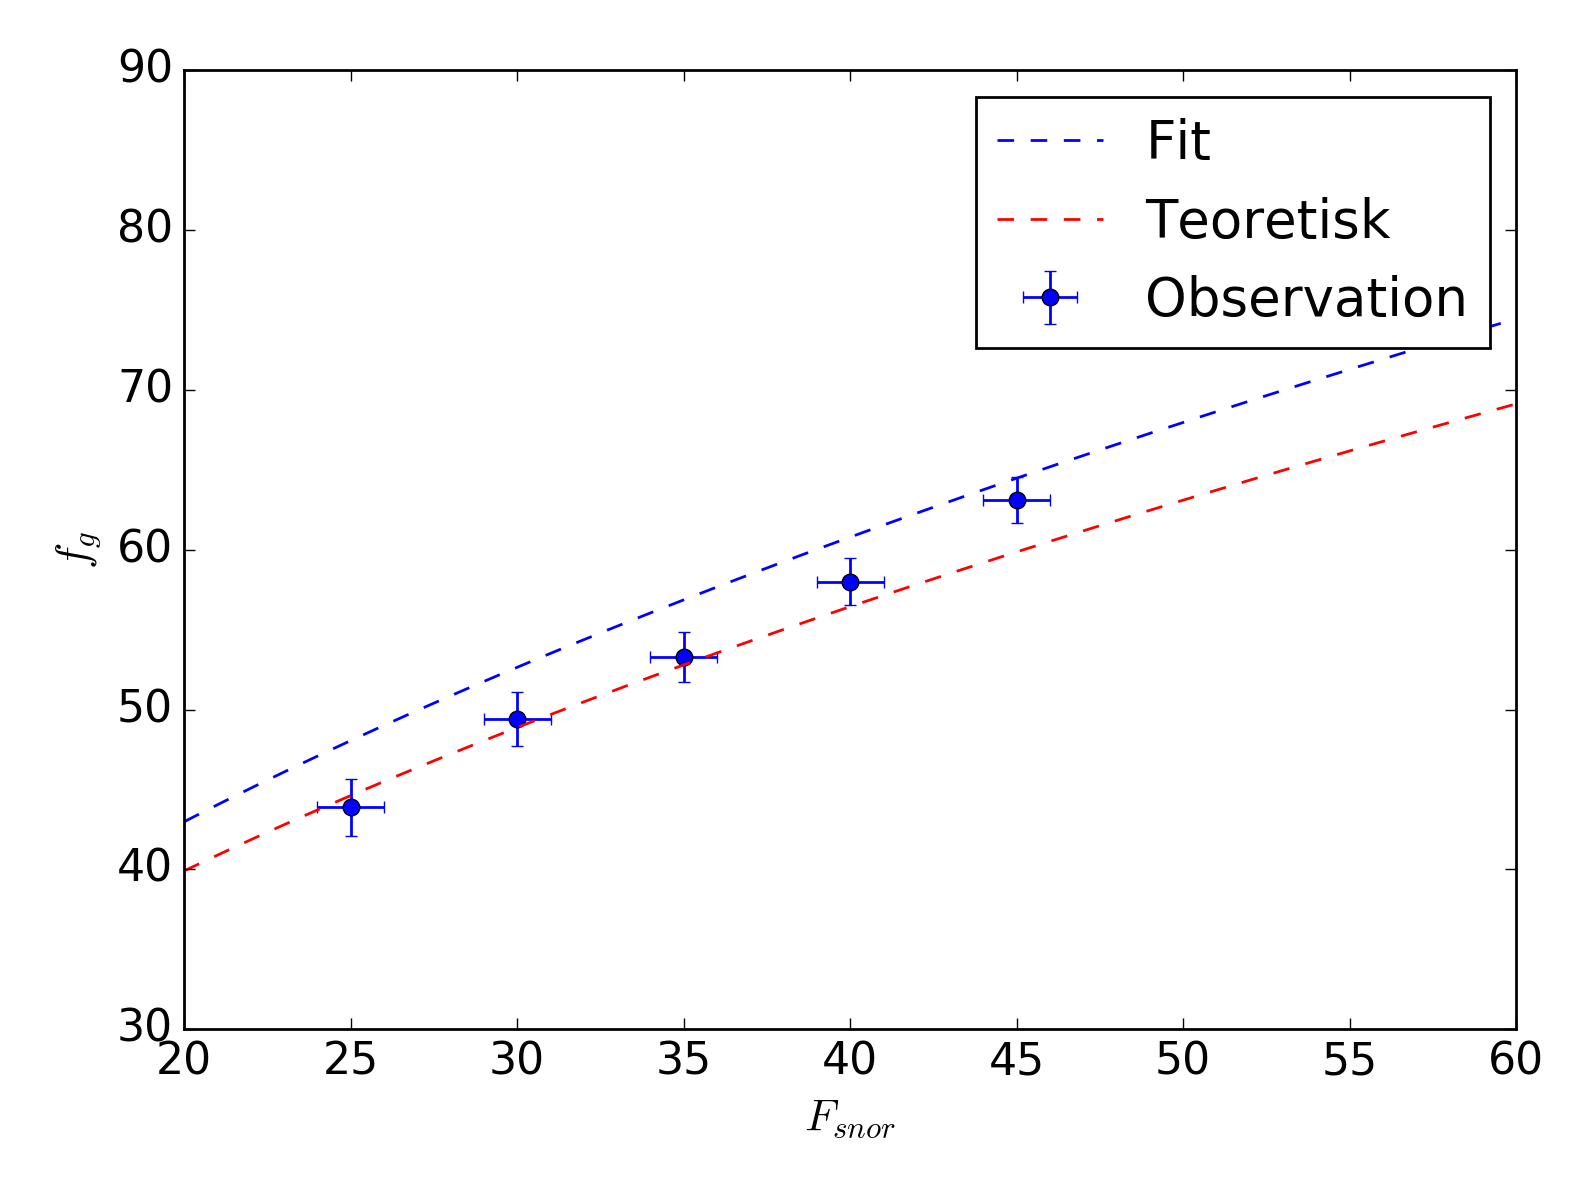
\includegraphics[width=\linewidth]{frekvensSnorSpaending.png}
    \caption{Resultater af fit, teoretisk værdier og observation af grundfekvensen som funktion af snorspændingen.}
    \label{fig:frekvensSNor}
\end{figure}

\subsection{Grundfrekvensens afhængighed af masse/længde}
Igen foretages varibel kontrol af samme \cref{eq: wave} Hvor snorspændingen $F$ og længden $L$ holdes konstant.
\begin{figure}[H]
    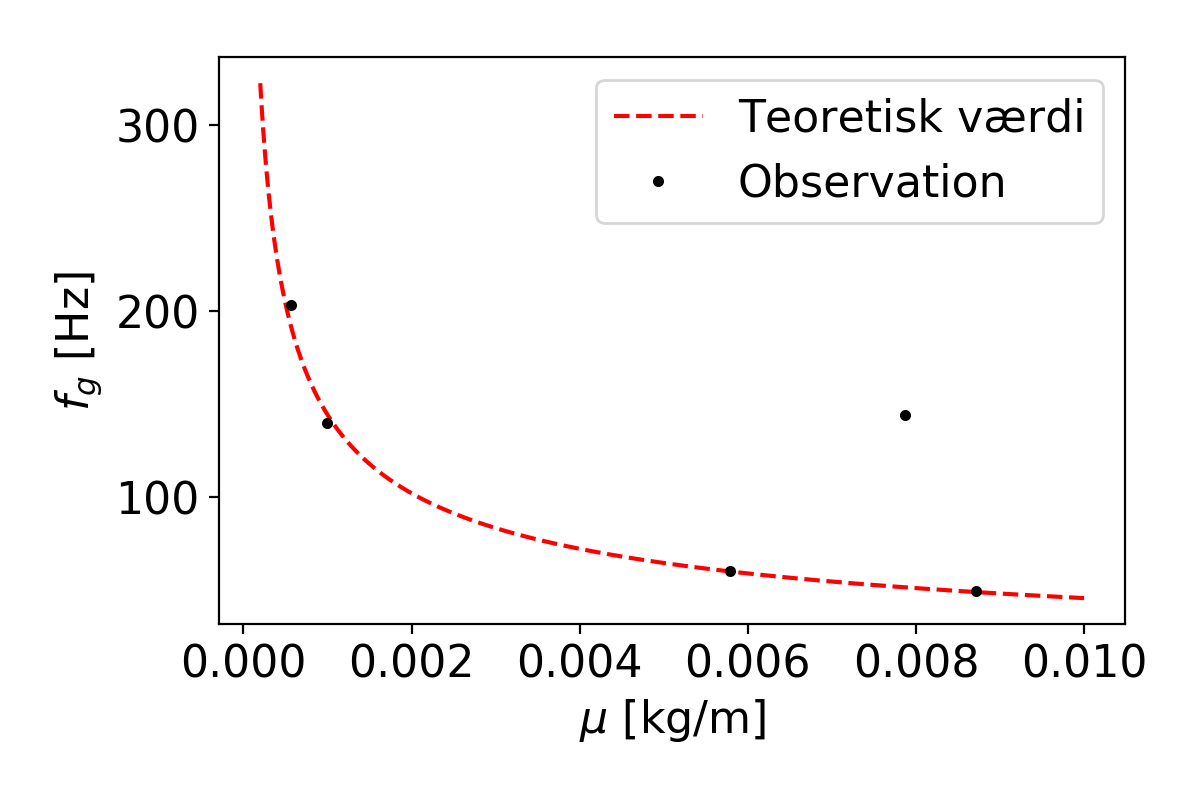
\includegraphics[width=\linewidth]{frekvensMu.png}
    \caption{Resultater af observationer og teoretiske værdier, af grundfrekvensen som funktion af snorspændingen.}
    \label{fig:frekvensMu}
\end{figure}


\end{document}
